\chapter{先看见磁岛，再建立撕裂模的方程}\label{tm:foundations}
\section{本讲义到底要回答什么}
撕裂模（tearing mode）是\textbf{电流片的拓扑改变型不稳定性}：一个很小的磁通扰动，在某些平衡中会自行增长，使原来从一端延伸到另一端的磁面分裂为磁岛。这里的“自行”是相对于持续外部强迫而言；能量来自原平衡的磁场与电流分布。电阻打开原先被理想磁冻结禁止的演化通道，并不作为供能电池。

有三个问题必须分开。第一，给定平衡是否有允许增长的扰动？这是\emph{稳定性}。第二，扰动以多快的速度长大、磁岛多宽？这是\emph{增长率与非线性演化}。第三，整个系统每秒重联多少磁通？这是\emph{重联率}。一个正增长率不等于最终稳态重联率，观察到一个磁岛也不能单独反推出线性增长率。

我们从最可控的二维、不可压、电阻MHD问题出发，真正算完外区解、内区尺度与两者的匹配。经典来源是Furth、Killeen与Rosenbluth的电阻撕裂研究；现代写法也可逐式对照Fitzpatrick的作者讲义。\citep{TMFKR1963,TMFitzMatching} 后文再说明该模型与实验、Hall模型和动理学模型的接口，而不把经典电阻标度误当成所有实验的答案。

\section{坐标、方向与量纲：全文固定这一套约定}
令$x$为穿过电流片的方向，$y$为沿电流片的方向，$z$为忽略变化的方向：$\partial_z=0$。平衡重联场沿$y$，可另有常数导场$B_g\hat{\vct z}$。取
\begin{equation}
 \B_\perp=\hat{\vct z}\times\nabla\psi
 =(-\partial_y\psi,\partial_x\psi,0),\qquad
 \vct u_\perp=\hat{\vct z}\times\nabla\phi
 =(-\partial_y\phi,\partial_x\phi,0).
 \label{tm:fluxstream}
\end{equation}
$\psi$是磁通函数，单位$\mathrm{T\,m}$；$\phi$是流函数，单位$\mathrm{m^2\,s^{-1}}$。\textbf{本讲义不是取$\B=\nabla\psi\times\hat{\vct z}$。}这两种约定只差整体符号，但若混用，欧姆律、X点电场和相位关系都会出错。

为什么引入两个看似抽象的函数？首先，
\begin{equation}
 \nabla\cdot\B_\perp=-\partial_x\partial_y\psi+\partial_y\partial_x\psi=0,
 \qquad \nabla\cdot\vct u_\perp=0.
\end{equation}
它们自动满足无磁单极与二维不可压约束。其次，
\begin{equation}
 \B_\perp\cdot\nabla\psi
 =-\psi_y\psi_x+\psi_x\psi_y=0.
\end{equation}
因此平面磁力线就是$\psi=\text{常数}$的等值线。作一张$\psi$的等高线图，就能看见拓扑；不必先数值追踪成千上万条粒子轨道。\textbf{磁力线也不是粒子轨道。}

定义泊松括号
\begin{equation}
 [f,g]\equiv\partial_x f\,\partial_y g-\partial_y f\,\partial_x g.
 \label{tm:bracket}
\end{equation}
它只是两项乘积之差，不要求读者预先学习Hamilton力学。逐项代入式\eqref{tm:fluxstream}可得
\begin{equation}
 \vct u\cdot\nabla g=(-\phi_y)g_x+\phi_xg_y=[\phi,g],
 \qquad \B_\perp\cdot\nabla g=[\psi,g].
\end{equation}
在后面的方程中看到括号，首先把它读成“沿流场/磁场的空间变化”。

忽略位移电流的Amp\`ere定律和二维涡量给出
\begin{align}
 \mu_0J_z&=\partial_xB_y-\partial_yB_x
 =\partial_x^2\psi+\partial_y^2\psi=\nabla_\perp^2\psi,\label{tm:current}\\
 \omega_z&=\partial_xu_y-\partial_yu_x=\nabla_\perp^2\phi.
 \label{tm:vorticity}
\end{align}
磁通函数的二阶导数控制电流；流函数的二阶导数控制涡量。撕裂层之所以薄而重要，正因为一个很小的磁通变化也可能具有很大的二阶导数。

\begin{center}
\begin{tabular}{lll}\toprule
符号&定义&SI单位\\\midrule
$\eta$&电阻率，$\E+\vct u\times\B=\eta\J$&$\Omega\,\mathrm m$\\
$D_\eta=\eta/\mu_0$&磁扩散系数&$\mathrm{m^2/s}$\\
$\rho$&质量密度，氢等离子体常取$m_in$&$\mathrm{kg/m^3}$\\
$a$&平衡电流片的特征半厚&$\mathrm m$\\
$\delta$&线性非理想内层的特征尺度&$\mathrm m$\\
$W$&磁岛\textbf{全宽}，不是半宽&$\mathrm m$\\
$k,\lambda=2\pi/k$&沿片波数、波长&$\mathrm{m^{-1}},\mathrm m$\\
$\gamma$&振幅的线性增长率&$\mathrm{s^{-1}}$\\\bottomrule
\end{tabular}
\end{center}
不少论文把磁扩散系数也写成$\eta$。每次读到$S=aV_A/\eta$，必须先检查该文$\eta$的单位；直接把$\Omega\,\mathrm m$代入这个式子，会漏掉$\mu_0$。

\section{用一个解析磁通函数算出X点、O点和岛宽}
在片中心附近，假设平衡$B_y\simeq B'_0x$，其中$B'_0>0$是中心磁场梯度，单位$\mathrm{T/m}$。积分$B_y=\psi_x$得$\psi_0=B'_0x^2/2$。加入沿$y$变化的正振幅扰动$\widetilde\psi>0$：
\begin{equation}
 \psi(x,y)=\frac{B'_0x^2}{2}+\widetilde\psi\cos(ky).
 \label{tm:islandpsi}
\end{equation}
于是$B_x=k\widetilde\psi\sin(ky)$，$B_y=B'_0x$。平面磁场为零必须同时满足$x=0$和$\sin(ky)=0$。

在$(x,y)=(0,0)$附近，$\cos(ky)\simeq1-k^2y^2/2$，故
\begin{equation}
 \psi-\widetilde\psi\simeq\frac{B'_0x^2}{2}-\frac{\widetilde\psi k^2y^2}{2}.
\end{equation}
等值线是双曲线，两条分离线相交，因此这是X点。在$(0,\pi/k)$附近，令$Y=y-\pi/k$，$\cos(ky)\simeq-1+k^2Y^2/2$，得到
\begin{equation}
 \psi+\widetilde\psi\simeq\frac{B'_0x^2}{2}+\frac{\widetilde\psi k^2Y^2}{2}.
\end{equation}
等值线是闭合椭圆，因此这是O点。常数导场不改变这张平面投影图，但在三维中磁力线沿$z$前进，磁岛截面对应磁通绳，不能说总磁场必在O/X点为零。

分离线通过X点，故其磁通值为$\psi_X=\widetilde\psi$。沿O点所在的$y=\pi/k$截线，分离线位置满足
\begin{equation}
 \frac{B'_0x^2}{2}-\widetilde\psi=\widetilde\psi
 \quad\Rightarrow\quad
 x=\pm2\sqrt{\frac{\widetilde\psi}{B'_0}}.
\end{equation}
上下两边之差就是全宽：
\begin{equation}
 \boxed{W=4\sqrt{\frac{\widetilde\psi}{B'_0}}},\qquad
 \psi_X-\psi_O=2\widetilde\psi=\frac{B'_0W^2}{8}.
 \label{tm:width}
\end{equation}
这个平方根关系极其重要：若磁通振幅按$e^{\gamma t}$增长，岛宽按$e^{\gamma t/2}$增长，二者的半对数图斜率差一倍。\citep{TMFitzIsland}

\paragraph{算完一个例子。}
取教学参数$B'_0=2\,\mathrm{T/m}$、$\widetilde\psi=5\times10^{-5}\,\mathrm{T\,m}$，则
\begin{equation}
 W=4\sqrt{2.5\times10^{-5}}\,\mathrm m=0.020\,\mathrm m=2.0\,\mathrm{cm}.
\end{equation}
若$k=20\,\mathrm{m^{-1}}$，波长$\lambda=2\pi/20=0.314\,\mathrm m$，扰动法向磁场峰值为$k\widetilde\psi=1.0\,\mathrm{mT}$。因此一个厘米级磁岛可以只对应毫特斯拉量级的法向磁扰动。由测量磁扰动反演岛宽，仍须知道$k$、磁剪切和诊断所在位置。

\begin{figure}[htbp]
\centering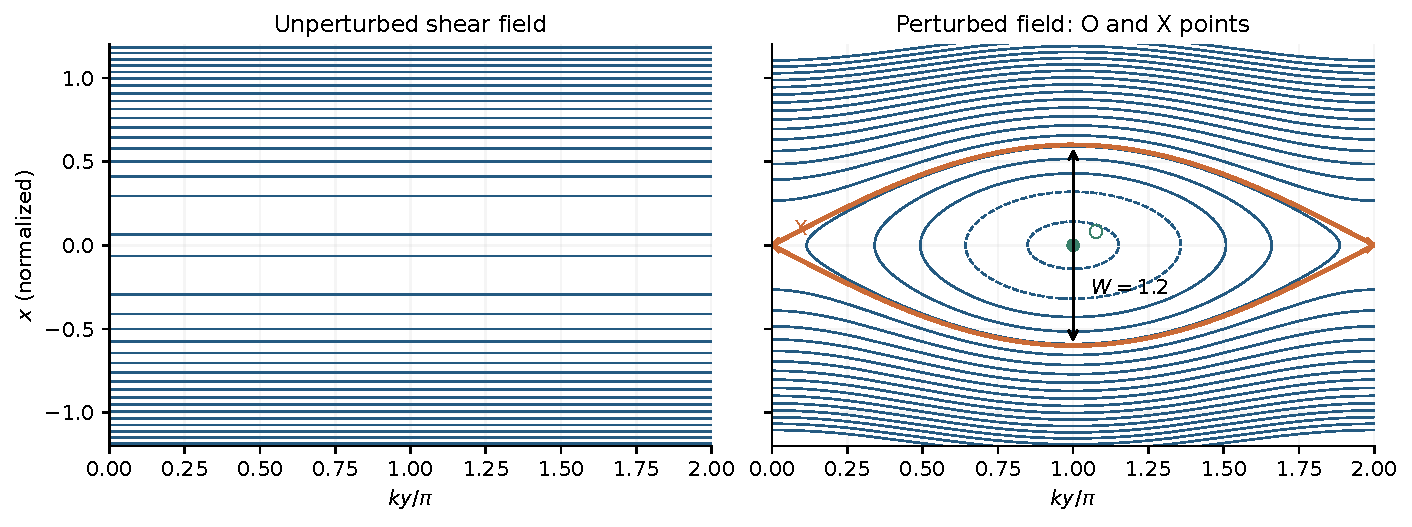
\includegraphics[width=\textwidth]{figures/tm_island.pdf}
\caption{由解析磁通函数直接绘制的磁岛。图采用无量纲$\psi=x^2/2+0.09\cos y$，所以全宽$W=4\sqrt{0.09}=1.2$。平面等值线、X/O点与分离线来自同一函数；这是教学解析图，不是实验照片或数值重联模拟。}
\label{tm:fig:island}
\end{figure}

\section{从MHD到磁通方程：不跳过符号}
从不可压、均匀密度、无黏性、标量电阻率的电阻MHD出发：
\begin{align}
 \rho(\partial_t\vct u+\vct u\cdot\nabla\vct u)&=-\nabla p+\J\times\B,\label{tm:momMHD}\\
 \E+\vct u\times\B&=\eta\J,\label{tm:ohmMHD}\\
 \partial_t\B&=-\nabla\times\E,\quad
 \mu_0\J=\nabla\times\B,\quad\nabla\cdot\B=0.
\end{align}
其中$\rho$为常数，$p$在不可压模型中负责维持$\nabla\cdot\vct u=0$；本章并未自洽计算温度。先这样简化，是为了单独看清电阻、惯性与磁剪切的作用，绝不是断言实验中的热流、黏性和双流体项总可忽略。

取矢势$A_z=-\psi$，则$\B=\nabla\times(-\psi\hat{\vct z})+B_g\hat{\vct z}$恰好符合式\eqref{tm:fluxstream}。由$\E=-\partial_t\vct A-\nabla\Phi_{\rm el}$，在$\partial_z\Phi_{\rm el}=0$规范下，$E_z=\partial_t\psi$。再逐项计算
\begin{equation}
 (\vct u\times\B)_z=u_xB_y-u_yB_x
 =-\phi_y\psi_x+\phi_x\psi_y=[\phi,\psi].
\end{equation}
将它与式\eqref{tm:current}代入欧姆律$z$分量，得
\begin{equation}
 \boxed{\partial_t\psi+[\phi,\psi]=D_\eta\nabla_\perp^2\psi.}
 \label{tm:induction}
\end{equation}
无电阻时右端为零，说明$\psi$被流场平流：$D\psi/Dt=0$。有电阻时，磁通可以相对于该流场改变。

可以给$\psi$加上只依赖时间的常数，磁场不变而$E_z$参考值改变；固定边界电压后该自由度也被固定。\textbf{二维重联的规范稳健量是X点与参考O点的磁通差。}移动的X/O点处$\nabla\psi=0$，所以
\begin{equation}
 \frac{\dd}{\dd t}(\psi_X-\psi_O)=E_z(X)-E_z(O).
 \label{tm:fluxrate}
\end{equation}
只有在参考电场可忽略或已明确扣除时，才可直接把$E_z(X)$叫作重联率。线性模的增长率$\gamma$则满足$\partial_t\widetilde\psi=\gamma\widetilde\psi$；它的单位是逆时间，不是电场单位。

\section{从动量方程到涡量方程：压力怎样被消去}
取式\eqref{tm:momMHD}的旋度。任意光滑标量满足$\nabla\times\nabla p=0$，因而压力梯度消失，但压力的力平衡作用没有被物理删除。二维不可压流的涡量沿$z$，没有涡量拉伸项，故惯性部分为
\begin{equation}
 \left[\nabla\times(\partial_t\vct u+\vct u\cdot\nabla\vct u)\right]_z
 =\partial_t\omega_z+\vct u\cdot\nabla\omega_z.
\end{equation}
这一等式也可用恒等式$\vct u\cdot\nabla\vct u=\nabla(u^2/2)-\vct u\times(\nabla\times\vct u)$逐项验证。

对磁力，在常数导场及仅有$J_z$的二维模型中，
\begin{equation}
 \J\times\B=J_z\hat{\vct z}\times(\hat{\vct z}\times\nabla\psi)
 =-J_z\nabla\psi.
\end{equation}
其旋度的$z$分量为
\begin{align}
 [\nabla\times(-J_z\nabla\psi)]_z
 &=-\partial_x(J_z\psi_y)+\partial_y(J_z\psi_x)\\
 &=-(J_{z,x}\psi_y+J_z\psi_{xy})+(J_{z,y}\psi_x+J_z\psi_{yx})\\
 &=\psi_xJ_{z,y}-\psi_yJ_{z,x}=[\psi,J_z].
\end{align}
两个含混合二阶导数的项恰好抵消。因此
\begin{equation}
 \boxed{\partial_t\nabla_\perp^2\phi+[\phi,\nabla_\perp^2\phi]
 =\frac{1}{\mu_0\rho}[\psi,\nabla_\perp^2\psi].}
 \label{tm:vortEq}
\end{equation}
式\eqref{tm:induction}和\eqref{tm:vortEq}构成下面使用的两场体系。二维不可压、常数导场情形下，它们直接来自上述MHD；在强导场、各向异性排序的三维问题中也会出现相关的约化MHD形式，但不能反过来把这两条二维式当成完整三维方程。\citep{TMLoureiro2007}

\section{选一个真正满足力平衡的电流片}
令
\begin{equation}
 B_{0y}(x)=B_0\tanh(x/a),\quad
 \psi_0(x)=B_0a\ln\cosh(x/a),\quad \phi_0=0.
 \label{tm:Harris}
\end{equation}
这里$B_0$是远离片中心的重联场，不是总导场。因为$\dd(\ln\cosh s)/\dd s=\tanh s$，第二式求导立即返回第一式。电流为
\begin{equation}
 J_{0z}(x)=\frac{B_0}{\mu_0a}\operatorname{sech}^2(x/a).
\end{equation}
再看$x$方向动量平衡：$0=-p_0'-J_{0z}B_{0y}$。用$J_{0z}=B_{0y}'/\mu_0$得
\begin{equation}
 \frac{\dd}{\dd x}\left(p_0+\frac{B_{0y}^2}{2\mu_0}\right)=0.
\end{equation}
因此
\begin{equation}
 p_0(x)=p_\infty+\frac{B_0^2}{2\mu_0}\operatorname{sech}^2(x/a).
\end{equation}
片中心磁压减少的部分被热压补上。常数导场只给总压增加常数，不改变这一平衡。

\paragraph{一个经常被省略的限制。}
在$D_\eta\ne0$且$\phi_0=0$时，$\partial_t\psi_0=D_\eta\psi_0''$，所以这不是永久静止的\emph{电阻}平衡。我们采用“冻结的背景近似”：平衡扩散时间$\tau_R=a^2/D_\eta$远长于模增长时间$\gamma^{-1}$。也可以明确加外源维持平衡，但那是另一种问题设定。后面必须检验$\gamma\tau_R\gg1$，而不能默默把平衡永远固定。

\section{归一化的每一个因子}
定义$V_A=B_0/\sqrt{\mu_0\rho}$、$\tau_A=a/V_A$，并令
\begin{equation}
 X=x/a,\quad Y=y/a,\quad \hat t=t/\tau_A,\quad
 \hat\psi=\psi/(B_0a),\quad \hat\phi=\phi/(V_Aa).
\end{equation}
磁通方程的时间项、平流项都具有量级$B_0V_A$，扩散项量级为$D_\eta B_0/a$。除以前者，得到系数
\begin{equation}
 \frac{D_\eta B_0/a}{B_0V_A}=\frac{D_\eta}{aV_A}=S_a^{-1},
 \qquad S_a\equiv\frac{aV_A}{D_\eta}=\frac{\tau_R}{\tau_A}.
\end{equation}
涡量方程两侧共同量级$V_A^2/a^2$，因为$B_0^2/(\mu_0\rho)=V_A^2$。故无量纲方程为
\begin{align}
 \partial_{\hat t}\hat\psi+[\hat\phi,\hat\psi]&=S_a^{-1}\hat\nabla_\perp^2\hat\psi,\\
 \partial_{\hat t}\hat\nabla_\perp^2\hat\phi+[\hat\phi,\hat\nabla_\perp^2\hat\phi]
 &=[\hat\psi,\hat\nabla_\perp^2\hat\psi].
\end{align}
这一步的实际作用是减少独立参数。改变$a,B_0,\rho,D_\eta$，只要$S_a$及边界、归一化波数相同，所选简化模型具有相同的无量纲线性问题；但真实等离子体的$d_i/a$、$\rho_i/a$与碰撞率可能同时改变，所以不能只看$S_a$就断言实验相似。
